% llama-modchip v3.2.0 Technical Paper (arXiv-compatible LaTeX2e source)
\documentclass[10pt,twocolumn]{article}

\ifdefined\pdfsuppressptexinfo
  \pdfsuppressptexinfo=15
\fi

\ifdefined\XeTeXversion
  % XeTeX / Tectonic natively handles UTF-8
\else
  \usepackage[utf8]{inputenc}
\fi
\usepackage[T1]{fontenc}
\usepackage{lmodern}
\usepackage[htt]{hyphenat}
\usepackage{microtype}
\usepackage[margin=0.72in]{geometry}
\usepackage{amsmath,amssymb,amsfonts,amsthm}
\usepackage{booktabs}
\usepackage{array}
\usepackage{tabularx}
\usepackage{multirow}
\usepackage{graphicx}
\usepackage{xcolor}
\usepackage{placeins}
\usepackage{xurl}
\usepackage{hyperref}

\hypersetup{
    colorlinks=true,
    linkcolor=blue!60!black,
    citecolor=blue!60!black,
    urlcolor=blue!70!black,
    pdftitle={llama-modchip v3.2.0: Three-Tier Donor-Free MaxQ Compression, Quantized Split-KV Decode, Native HARP-Cache v2, and RouteCrack 2.0 L1 Micro-Arbiter Speculative Decoding},
    pdfauthor={Paolo Colombo}
}

\newtheorem{proposition}{Proposition}
\newtheorem{remark}{Remark}

\setlength{\columnsep}{0.24in}
\tolerance=2000
\emergencystretch=3em
\hfuzz=1pt
\newcolumntype{L}{>{\raggedright\arraybackslash}X}

\title{\textbf{\Large \texttt{llama-modchip v3.2.0}: Three-Tier Donor-Free \texttt{MaxQ} Compression, Zero-Collision Multi-ISA Kernels, Quantized Split-KV Decode, and \texttt{RouteCrack 2.0} Speculative Decoding}}

\author{
  \textbf{Paolo Colombo} \\
  Independent Systems \& Machine Learning Researcher \\
  \texttt{synchopate@gmail.com} \quad $\cdot$ \quad \texttt{https://github.com/synchopate/llama-modchip}
}

\date{November 2026}

\begin{document}

\maketitle

\begin{abstract}
Running 30B--284B Sparse Mixture-of-Experts (MoE) language models on commodity 16--64~GB CPU workstations is constrained by Per-Layer Embedding (PLE) capacity, DDR5 memory bandwidth, and speculative decoding overhead. Standard 2-bit quantizers either exceed 32--64~GB RAM budgets or rely on lossy expert pruning and donor weight copying, while multi-step neural draft loops burn milliseconds on large-vocabulary \texttt{lm\_head} projections or over-draft high-entropy text on bandwidth-bound MoE backends.

We present \texttt{llama-modchip v3.2.0}, an open-source inference architecture uniting three co-designed layers: (1) a Three-Tier Donor-Free \texttt{MaxQ} Fleet spanning 64~GB (\texttt{Qwen3.8 MaxQ-64GB}, 53.99~GiB, blind \texttt{wiki-alt.txt} PPL 3.4325, $-46.6\%$ KLD vs.\ a 54.40~GiB coder-pruned \texttt{IQ1\_M} baseline, cold-cache Cgroup v2 certified at 48.35~GiB $\le 60$~GiB with \texttt{pgsteal=0}, \texttt{Swap=0}; \texttt{DeepSeek-V4 284B MaxQ-v4}, 57.99~GiB, 6.8592 PPL, $\approx 60.5$~GiB working set), 32~GB (\texttt{Qwen3.8 MaxQ-32GB}, 24.98~GiB trunk + 10.73~GiB lazy NVMe \texttt{PCA-Wiener}+\texttt{RaBitQ} \mbox{\texttt{Q1\_0}} PLE, cold-cache Cgroup v2 certified at 28.26~GiB $\le 28.5$~GiB, \texttt{pgsteal=0}, $>10.5$~GiB PLE unfaulted), and 16~GB (\texttt{Nemotron-3.5-30B MaxQ-16GB}, 13.39~GiB, $N=1$ fitting ${\approx}15$~GiB; plus \texttt{VQ3-64} 13.30~GiB and \texttt{Fractal-64} 14.36~GiB); (2) a Zero-Collision \texttt{ggml} ABI preserving upstream types 41--43 with \texttt{FRACTAL\_64} (3.75~bpw) at 44 and \texttt{VQ3\_64} (3.00~bpw) at 45 across AVX-512, AVX2, NEON, and Metal plus zero-copy 3D MoE \texttt{{-}{-}repack}, \textbf{Quantized \& Heterogeneous Split-KV Decode} ($+15.1\%$ to $+61.4\%$ at 32K on \texttt{Q8\_0/Q4\_0} KV with ${\sim}2\times 10^{-8}$ parity), and \textbf{Native C++ Chained-Prefix HARP-Cache v2} (O($L/256$) Radix lookup + 16.40~ms \texttt{/dev/shm} post-restart restore); and (3) \texttt{RouteCrack 2.0} (\texttt{{-}{-}spec-type routecrack2}), fusing NextN MTP/\texttt{RCPredictor}, O(1) Two-Zone 40K Suffix bypass ($<250$~ns), and 192~KB Stockfish-PVS Zobrist memory under an 832~B L1-resident \texttt{[10$\to$16$\to$1]} SIMD Micro-Arbiter. On 16 Zen~5 cores (0~GPU), \texttt{RouteCrack 2.0} reaches 15.34~tok/s uncapped (15.64$\pm$0.05 in cold 60~GiB cgroup; 21.38--22.00 \texttt{W1}) on aligned \texttt{Qwen3.8-MaxQ-64GB}, 7.79 (12.31 \texttt{W1}) on \texttt{DeepSeek-V4 MaxQ-v4}, and 28.20 (42.18 \texttt{W1}) on \texttt{Nemotron-30B} (\texttt{Fractal-MXFP4} ref).
\end{abstract}

\section{Introduction}

Sparse Mixture-of-Experts (MoE) architectures paired with hybrid linear-attention, state-space, or latent-attention compression decouple total parameter capacity from per-token active FLOPs. Three open-weights model families span the current local deployment spectrum:
\begin{enumerate}
    \item \textbf{\texttt{Qwen3.8-Flash-Next}} \cite{qwen38} ($176.5\text{B}$ total, $5\text{B}$ active): A 48-layer hybrid architecture combining 36 \texttt{Gated DeltaNet} (GDN) linear-attention layers, 12 Grouped-Query Attention (GQA) layers, 512 routed experts per layer, a $320\text{M}$-row Per-Layer Embedding (PLE) table, a $248\text{K}$-token vocabulary, and a built-in \texttt{blk.48} 1-layer NextN Multi-Token Prediction (MTP) module \cite{gloeckle2024mtp}.
    \item \textbf{\texttt{DeepSeek-V4-Flash-0731}} \cite{deepseekv4,deepseekv3} ($284.33\text{B}$ total, $13.17\text{B}$ active): A 43-layer MoE Transformer combining 64-head Multi-Head Latent Attention (MLA, compressed KV latent rank 512, query LoRA rank 1024, 8 output head-groups of rank 1024), sparse \texttt{CSA}/\texttt{LID}/\texttt{HCA} indexer compressors, 4-stream Sinkhorn-20 Hyper-Connections, and 256 routed experts (top-6 active plus 1 shared expert, with deterministic hash routing \texttt{tid2eid} on layers $0..2$).
    \item \textbf{\texttt{NVIDIA-Nemotron-3.5-Lightning-30B-A3B}} \cite{nemotron35,nemotron2025} ($30.2\text{B}$ total, $3.0\text{B}$ active): A 52-layer hybrid architecture comprising 23 Mamba-2 State-Space Model (SSM) layers, 23 Sparse MoE layers (128 routed experts, top-6 active + 1 shared expert), and 6 GQA layers.
\end{enumerate}

Running all three families cleanly inside 16~GB, 32~GB, and 64~GB commodity workstations on top of \texttt{llama.cpp} \cite{llamacpp} exposes four fundamental engineering walls:
\begin{itemize}
    \item \textbf{The Donor-Free Capacity Wall}: Across 18 third-party \texttt{Qwen3.8-Flash-Next} GGUF checkpoints published on Hugging Face (54.40--329.72~GiB), $0/18$ fit inside a 28.5~GiB budget because leaving the 320M-row PLE table in \texttt{IQ4\_NL} consumes 26.82~GiB alone, leaving $<1.7$~GiB for the 48-layer MoE trunk; similarly, uncalibrated 2-bit \texttt{DeepSeek-V4} builds either exceed 64~GiB or degrade severely.
    \item \textbf{ABI Fragmentation Across Quantization Formats}: Repurposing upstream \texttt{ggml} type enum slots breaks binary compatibility whenever upstream introduces standard formats such as \texttt{GGML\_TYPE\_Q1\_0} (41), \texttt{GGML\_TYPE\_Q2\_0} (42), or \texttt{GGML\_TYPE\_F8\_E4M3} (43).
    \item \textbf{CPU-MoE Speculative Cost Asymmetry}: On 1-layer NextN MTP models (\texttt{Qwen3.8}), chaining sequential \texttt{draft-mtp} steps incurs $3\times{\sim}15$~ms of $248\text{K}$ \texttt{lm\_head} compute without suffix memory; conversely, on 284B non-MTP MoE models, drafting unverified prose tokens streams additional routed experts from DDR5 at $+0.395\times T_1$ latency per step.
    \item \textbf{3D MoE Repack Memory Blowup \& Barrier Convoys}: Default heap repacking on 3D MoE tensors (\texttt{ne[2] >= 64}) destroys zero-copy \texttt{mmap} sharing (inflating \texttt{RssAnon} $5.4\times$ to 9.81~GiB), while oversubscribed \texttt{-t N {-}{-}poll 50} threads induce OS barrier convoys.
\end{itemize}

\begin{figure*}[t]
\centering
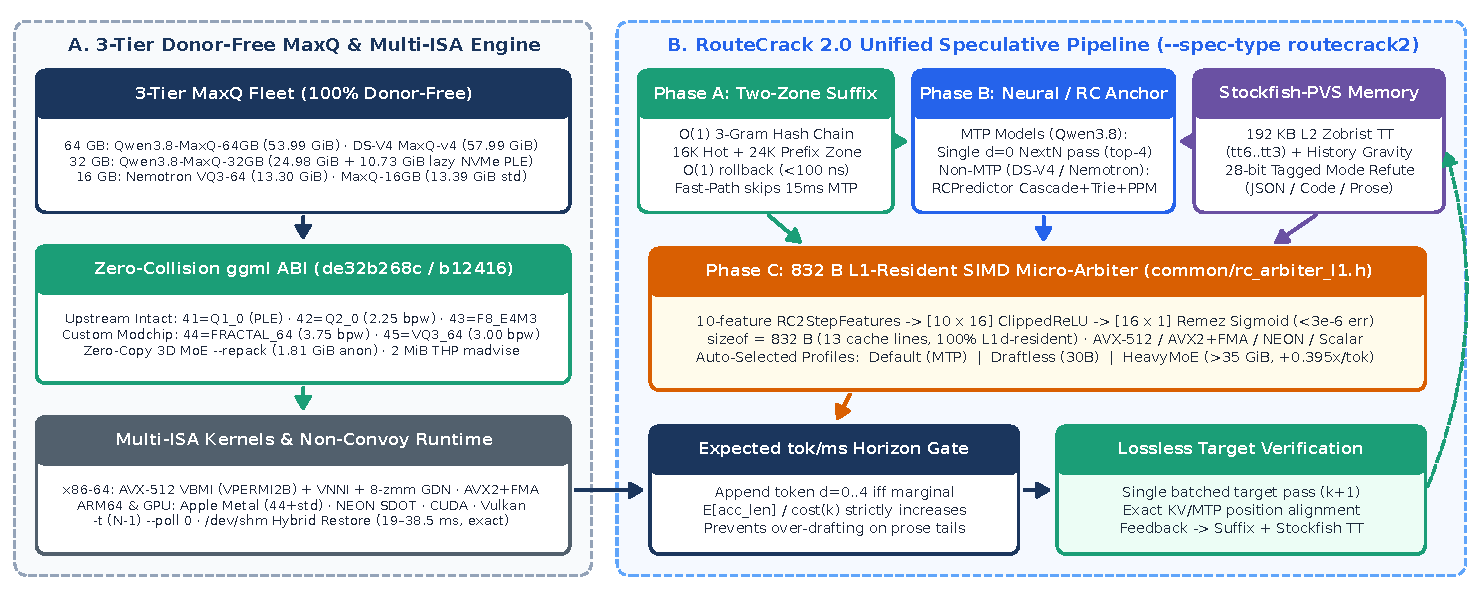
\includegraphics[width=\textwidth]{figures/fig1_routecrack2_architecture.pdf}
\caption{End-to-end \texttt{llama-modchip v3.2.0} architecture. (A) Three-tier donor-free \texttt{MaxQ} fleet running over a zero-collision \texttt{ggml} ABI (\texttt{41..45}), multi-ISA SIMD/Metal kernels, Quantized Split-KV Decode, Native C++ HARP-Cache v2, and zero-copy 3D MoE \texttt{{-}{-}repack}. (B) Unified \texttt{RouteCrack 2.0} speculative pipeline combining O(1) Two-Zone 40K Suffix bypass, Neural MTP/\texttt{RCPredictor} anchoring, 192~KB Stockfish-PVS Zobrist memory with 28-bit Tagged Mode Refutation, and an 832~B L1-resident SIMD Micro-Arbiter.}
\label{fig:arch}
\end{figure*}

Figure~\ref{fig:arch} summarizes our \texttt{v3.2.0} co-design. All modifications ship in a single unified patch (\texttt{patches/llama-modchip-v3.2.patch}) pinned to \texttt{llama.cpp @ 46eb1742d} (build \texttt{12604}, including native \texttt{inkling2.cpp}), compiling across Linux x86-64/ARM64, macOS Apple Metal, Windows 11 (MinGW/MSVC/CUDA), and Vulkan.

\section{Related Work}
\label{sec:related}

\paragraph{Post-Training \& Vector Quantization.}
Hessian-guided post-training quantization (GPTQ \cite{frantar2023gptq}), activation-aware scaling (AWQ \cite{lin2024awq}), and sensitivity-based dense-and-sparse non-uniform quantization (SqueezeLLM \cite{squeezellm}) achieve strong 3--4~bit dense fidelity, while lattice and multi-codebook vector quantizers such as QuIP\# \cite{tseng2024quip} and AQLM \cite{egiazarian2024aqlm} push toward 2~bits via incoherence processing or additive lookup tables. \texttt{MaxQ} adapts these ideas to 256--512-expert MoE blocks on CPU by (i) solving routed per-expert Hessians in FP64 via the Woodbury dual identity when $N_C \ll d_{\text{in}}$, (ii) pairing \texttt{PCA-Wiener} projection with \texttt{RaBitQ} \cite{rabitq2024} 1-bit quantization for massive PLE tables, and (iii) storing a 384~B 3D spherical Lloyd-Max codebook (\texttt{VQ3\_64}) entirely inside six AVX-512 \texttt{ZMM} registers decoded via \texttt{VPERMI2B}.

\paragraph{Local CPU/Hybrid Inference Systems.}
IO-aware exact GPU attention tiling (FlashAttention-2 \cite{dao2023flashattention2}) minimizes HBM traffic on GPUs, whereas consumer CPU/hybrid engines such as \texttt{llama.cpp} \cite{llamacpp}, PowerInfer \cite{powerinfer} (which exploits hot/cold ReLU neuron locality across GPU and CPU), and KTransformers \cite{ktransformers} (heterogeneous GPU attention + CPU MoE offloading) target memory-constrained workstations. \texttt{llama-modchip} builds directly atop \texttt{llama.cpp} to eliminate GPU dependence entirely where needed, adding register-stationary AVX-512 \texttt{MQA8} attention, zero-copy 3D MoE \texttt{{-}{-}repack}, inward 2~MiB THP alignment for lazy NVMe PLE paging, and a zero-collision \texttt{ggml} ABI.

\paragraph{Speculative Decoding.}
Standard speculative decoding \cite{leviathan2023fast} and learned multi-head/feature drafters such as Medusa \cite{cai2024medusa}, EAGLE \cite{li2024eagle}, and native NextN MTP \cite{gloeckle2024mtp} target GPU regimes where verifying $k$ draft tokens adds negligible latency. Draftless and retrieval-based methods---including Lookahead Decoding \cite{fu2024lookahead}, REST \cite{he2024rest}, Prompt Lookup Decoding \cite{saxena2023promptlookup}, and upstream \texttt{llama.cpp} \texttt{ngram-map-k} / \texttt{draft-mtp} \cite{llamacpp}---avoid a separate draft model but use fixed horizons or separate dispatch paths. \texttt{RouteCrack 2.0} explicitly models the non-zero CPU-MoE verification cost $\Delta C \in [0.285, 0.395]\,T_1$, unifying suffix lookup, single-pass MTP/\texttt{RCPredictor} anchoring, and Stockfish-style transposition tables \cite{stockfish} under an 832~B L1d-resident SIMD arbiter.

\section{Three-Tier Donor-Free \texttt{MaxQ} Compression \& Zero-Collision ABI}
\label{sec:quant}

\subsection{Zero-Collision \texttt{ggml} Type ABI (\texttt{41..45})}
To guarantee simultaneous compatibility with upstream \texttt{llama.cpp} formats and custom block-64 CPU/Metal kernels inside one binary, \texttt{llama-modchip v3.1.1} preserves all upstream enums untouched and places custom kernels at dedicated non-colliding IDs (Table~\ref{tab:abi}):
\begin{itemize}
    \item \textbf{Upstream Standard Types Preserved}: \texttt{GGML\_TYPE\_Q1\_0 = 41} (RaBitQ 1-bit PLE), \texttt{GGML\_TYPE\_Q2\_0 = 42} (18~B / 64~W $= 2.25$~bpw signed-scale), and \texttt{GGML\_TYPE\_F8\_E4M3 = 43}.
    \item \textbf{\texttt{Fractal-64} (\texttt{GGML\_TYPE\_FRACTAL\_64 = 44}, 30~B / 64~W $= 3.75$~bpw)}: Stores an FP16 super-scale $d$, eight 4-bit shifted sub-scales $\tilde{m}_s = m_s + 4 \in \{4..19\}$, and 64 3-bit indices into the kurtosis-matched dyadic codebook $\{-14,-8,-4,-1,+1,+4,+8,+14\}$. Achieves \textbf{17.75~dB SQNR} (99.15\% cosine similarity on raw \texttt{BF16} MoE weights, $+1.45$~dB over \texttt{Q3\_K}). Sub-scale multiplication fuses into \texttt{vpmaddwd} at zero extra instructions, \texttt{qh} unpacking uses AVX-512 \texttt{vprorvq}, and community-contributed register-tiled Apple Metal shaders (GitHub PR~\#24) sustain \textbf{78.60~tok/s} on M3 Max and \textbf{57.65~tok/s} on M1 Max.
    \item \textbf{\texttt{LUT-VQ3-64} (\texttt{GGML\_TYPE\_VQ3\_64 = 45}, 24~B / 64~W $= 3.00$~bpw)}: Encodes 60 weights as twenty 7-bit indices into a 128-entry 3D spherical Lloyd-Max codebook (384~B held across six AVX-512 \texttt{ZMM} registers) plus 4 tail weights and eight 3-bit sub-scales $\tilde{m}_s \in \{2..9\}$. Decoded in-register via three AVX-512 VBMI \texttt{VPERMI2B} (\texttt{\_mm512\_mask2\_permutex2var\_epi8}) lookups (with portable AVX2, ARM64 NEON, and scalar fallbacks), achieving \textbf{13.57~dB SQNR} ($+3.42$~dB over \texttt{Q2\_K}).
\end{itemize}

\begin{table}[t]
\centering
\caption{Zero-collision \texttt{ggml} type enum map in \texttt{llama-modchip v3.2.0} (\texttt{ggml/include/ggml.h} @ \texttt{46eb1742d}).}
\label{tab:abi}
\scriptsize
\setlength{\tabcolsep}{2.6pt}
\begin{tabularx}{\columnwidth}{@{}clccL@{}}
\toprule
\textbf{ID} & \textbf{Enum Symbol} & \textbf{B/64W} & \textbf{BPW} & \textbf{Origin / Backends} \\
\midrule
41 & \texttt{Q1\_0} & 10 & 1.25 & Upstream (AVX-512/AVX2/Metal/CUDA) \\
42 & \texttt{Q2\_0} & 18 & 2.25 & Upstream (AVX-512/AVX2/Metal/CUDA) \\
43 & \texttt{F8\_E4M3} & 64 & 8.00 & Upstream FP8 E4M3 (intact) \\
44 & \texttt{FRACTAL\_64} & 30 & 3.75 & Modchip (AVX-512/AVX2/NEON/Metal) \\
45 & \texttt{VQ3\_64} & 24 & 3.00 & Modchip (AVX-512 VBMI/AVX2/NEON) \\
\bottomrule
\end{tabularx}
\end{table}

\subsection{Three-Tier Donor-Free \texttt{MaxQ} Algorithms \& Loader Scope}
Every \texttt{v3.1.1} flagship checkpoint is quantized 100\% donor-free directly from upstream \texttt{BF16}/\texttt{MXFP4} weights with zero donor GGUF weight copying:
\begin{enumerate}
    \item \textbf{64~GB \& 32~GB \texttt{Qwen3.8-Flash-Next} (\texttt{MaxQ-64GB} \& \texttt{MaxQ-32GB}, std \texttt{ggml} types $\le 42$)}:
    Projecting the $320\text{M}$-row PLE table with \textbf{\texttt{PCA-Wiener} ($D=256$) + \texttt{RaBitQ Q1\_0}} \cite{rabitq2024} shrinks Shard~2 from 26.82~GiB (\texttt{IQ4\_NL}) to \textbf{10.73~GiB}, reinvesting $+16.09$~GiB into all 512/512 unpruned routed experts, \textbf{FP64 Woodbury DualGram} signed-scale \texttt{Q2\_0}, and the 0.81~GiB \texttt{blk.48} NextN MTP head. \texttt{MaxQ-64GB} (53.99~GiB, 0 ConeCollapse bias, 48.09~GiB \texttt{VmHWM} / 48.35~GiB cold cgroup peak $\le 60.0$~GiB at \texttt{-c 32768}, \texttt{pgsteal=0}; 45.08~GiB warm-cache gate \texttt{VmHWM}, \texttt{RssAnon = 1.81~GiB}) uses standard types $\le 42$ (pass \texttt{{-}{-}no-repack} on unpatched upstream \texttt{llama.cpp}; \texttt{llama-modchip v3.1.1} is recommended for zero-copy 3D MoE \texttt{{-}{-}repack} and \texttt{RouteCrack 2.0}). \texttt{MaxQ-32GB} adds 42-layer \textbf{\texttt{ConeCollapse}} intermediate width pruning ($K=640\to 512$ with post-quantization \texttt{F32} \texttt{ffn\_down\_exps.bias}, requiring the \texttt{llama-modchip v3.1.1+} loader), compressing Shard~1 to 24.98~GiB while demand-paging Shard~2 lazily from NVMe via \texttt{mmap} (\textbf{26.79~GiB} $N=1$ / \textbf{28.26~GiB} \texttt{RC2} cold-cache cgroup peak $\le 28.5$~GiB at \texttt{-c 32768} with \texttt{pgsteal=0}, \texttt{Swap=0}, and $>10.5$~GiB of PLE unfaulted---leaving a tight 0.24~GiB headroom at 32K context; 26.91--27.44~GiB in our warm-cache shorter-context gate).
    \item \textbf{64~GB \texttt{DeepSeek-V4-Flash-0731 MaxQ-v4} (57.99~GiB, 0 custom tensor types)}:
    Replaces custom MLA/Indexer formats with \texttt{0731}-imatrix-weighted standard \texttt{ggml} tensor types (446 2D K-quant projections, 9 full-width $K=2048$ ridge anchor layers, and 34 $K=1792$ \texttt{ConeCollapse} layers with $0.60\,\boldsymbol{\mu}$ shrunk residual bias and FP64 Woodbury DualGram $N_C=384$). Having zero custom tensor types enables native CPU, Apple Metal, CUDA, and Vulkan kernel execution inside \texttt{llama-modchip v3.1.1+}, while its 34 \texttt{ffn\_down\_exps.bias} tensors require \texttt{llama-modchip}'s \texttt{ConeCollapse} loader. At \texttt{-c 32768}, its total working set (${\approx}60.3$--$60.7$~GiB $= 57.99$~GiB weights $+ 2.25$--$2.67$~GiB anon) exceeds a strict 60.0~GiB cap (requiring $\ge 61$~GiB free RAM for zero-refault bare-metal residency); under a 60.0~GiB cgroup (\texttt{Swap=0}), it finishes without OOM via continuous ZFS-ARC-backed file reclaim (Section~\ref{sec:eval}).
    \item \textbf{16~GB \texttt{NVIDIA-Nemotron-3.5-30B-A3B} (\texttt{VQ3-64} 13.30~GiB, \texttt{Fractal-64} 14.36~GiB, \& \texttt{MaxQ-16GB} 13.39~GiB)}:
    \texttt{VQ3-64} (\texttt{types 44/45}) combines \texttt{Fractal-64} on boundary/down MoE layers with \texttt{LUT-VQ3-64} on 19 interior pre-\texttt{ReLU$^2$} up-projections (\texttt{wiki-alt} PPL \textbf{6.7614}, \texttt{WikiText-2} PPL \textbf{7.4400} vs.\ \texttt{BF16} \textbf{6.9582}), while \texttt{MaxQ-16GB} ($\max\text{type}=42$, 0 custom types, 0 ConeCollapse bias) targets unmodified upstream \texttt{llama.cpp} (\texttt{de32b268c+}) and downstream runners supporting \texttt{GGML\_TYPE\_Q2\_0 = 42}; under cold-cache 15.0~GiB Cgroup v2 (\texttt{-c 32768}, \texttt{Swap=0}), pure $N=1$ (${\approx}15.03$~GiB) nearly fits with 0.2~GiB refault, while \texttt{RC2} (${\approx}15.75$~GiB) requires $\ge 16$~GiB free RAM to avoid file reclaim (Section~\ref{sec:eval}).
\end{enumerate}

\begin{figure*}[t]
\centering
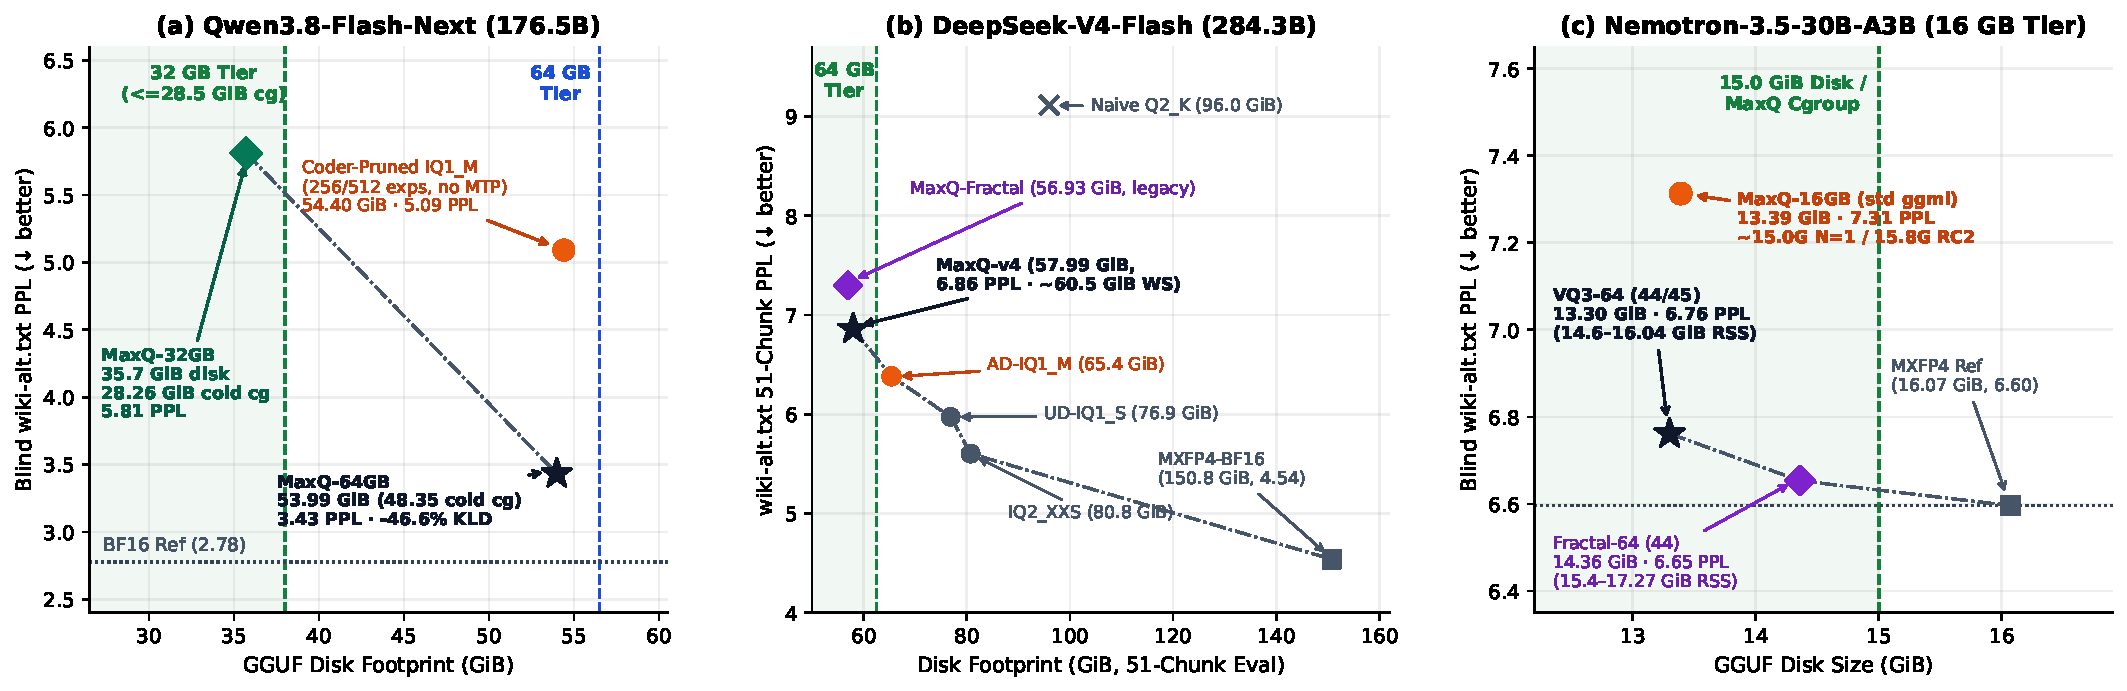
\includegraphics[width=\textwidth]{figures/fig2_pareto_frontier.pdf}
\caption{GGUF disk footprint vs.\ blind \texttt{wiki-alt.txt} perplexity Pareto frontier across all three RAM tiers (disk size on x-axis; cold-cache Cgroup v2 / working-set footprints annotated). (a) \texttt{Qwen3.8-Flash-Next} ($40\times 512$ blind chunks): \texttt{MaxQ-64GB} (53.99~GiB disk, 48.35~GiB cold cgroup peak $\le 60$~GiB, \texttt{pgsteal=0}) beats 54.40~GiB coder-pruned \texttt{IQ1\_M} (256/512 experts, no MTP) by $-1.66$~PPL ($-46.6\%$ KLD) while \texttt{MaxQ-32GB} (35.71~GiB disk, 28.26~GiB cold cgroup peak $\le 28.5$~GiB via 42L ConeCollapse + lazy NVMe PLE, \texttt{pgsteal=0}) keeps $>10.5$~GiB PLE unfaulted. (b) \texttt{DeepSeek-V4 284B} (51 chunks): donor-free \texttt{MaxQ-v4} (57.99~GiB disk, ${\approx}60.5$~GiB working set; requires $\ge 61$~GiB free) reaches 6.86~PPL. (c) \texttt{Nemotron-3.5 30B} ($40\times 512$): \texttt{MaxQ-16GB} $N=1$ fits ${\approx}15$~GiB (\texttt{RC2} needs ${\approx}15.75$~GiB), while \texttt{VQ3-64} (14.6--16.04~GiB RSS) and \texttt{Fractal-64} (15.4--17.27~GiB RSS) target 16--24~GB hosts.}
\label{fig:pareto}
\end{figure*}

Figure~\ref{fig:pareto} illustrates the resulting disk-footprint vs.\ perplexity Pareto frontier.

\section{Mathematical Co-Design: \texttt{Woodbury DualGram}, Low-Rank SVD, \& \texorpdfstring{$L_2$}{L2}-Quadrature MoE Pruning}
\label{sec:math}

\subsection{FP64 Woodbury DualGram \& \texttt{ConeCollapse}}
When quantizing a weight matrix $\mathbf{W} \in \mathbb{R}^{d_{\text{out}} \times d_{\text{in}}}$ against $N_C \ll d_{\text{in}}$ routed calibration activations $\mathbf{H}_c \in \mathbb{R}^{N_C \times d_{\text{in}}}$ (e.g., $N_C = 384$, $d_{\text{in}} = 2048$), forming the full $d_{\text{in}}\times d_{\text{in}}$ Hessian $\mathbf{H}_c^\top \mathbf{H}_c + \lambda \mathbf{I}$ is both ill-conditioned and costly across 256--512 experts per layer. Applying the Woodbury matrix identity reduces Hessian inversion to an $N_C \times N_C$ FP64 Cholesky dual solve:
\begin{equation}
    (\mathbf{H}_c^\top \mathbf{H}_c + \lambda \mathbf{I})^{-1} = \lambda^{-1}\!\left(\mathbf{I} - \mathbf{H}_c^\top (\mathbf{H}_c \mathbf{H}_c^\top + \lambda \mathbf{I}_{N_C})^{-1} \mathbf{H}_c\right),
\end{equation}
maintaining observed dual-Gram condition number $\kappa_2 \le 86.33$ during \texttt{MaxQ-v4} quantization while capturing cross-channel activation covariance. Under \texttt{ConeCollapse}, pruning low-energy intermediate channels ($K_{\text{full}} \to K_{\text{red}}$) is paired with a post-quantization shrunk residual centroid bias $\mathbf{b}_{\text{down}} = \gamma\,\mathbb{E}[\mathbf{W}_{\text{down}}\mathbf{h} - \widehat{\mathbf{W}}_{\text{down}}\hat{\mathbf{h}}]$ (\texttt{GGML\_OP\_ADD\_ID}), preserving downstream residual mean and variance across all 34--42 collapsed layers.

\subsection{Spectral Decay of \texorpdfstring{$\mathbf{W}_{o,b}\mathbf{W}_{o,a}$}{Wob Woa} \& \texorpdfstring{$L_2$}{L2}-Quadrature MoE Tail Pruning}
In \texttt{DeepSeek-V4-Flash}, 31.0\% of per-token DRAM traffic (991.6~MB/tok) traverses the unactivated MLA output chain $\mathbf{y}_{\text{attn}} = \sum_{g=1}^{8} \mathbf{W}_{o,b}^{(g)}(\mathbf{W}_{o,a}^{(g)} \mathbf{x}_g)$. Exact SVD reveals rapid spectral decay ($\sigma_0 = 15.398 \to \sigma_{768} = 0.901 \to \sigma_{1023} = 0.048$): rank-768 truncation ($-25\%$ DRAM) preserves 99.64\% of Frobenius energy and 0.998204 output cosine similarity.

For optional runtime MoE tail pruning on learned-router layers ($l \ge 3$, leaving hash-routed lexical layers $l \in \{0,1,2\}$ at full Top-6), let $\mathbf{y}_{\text{FFN}} = \mathbf{e}_{\text{shared}} + \sum_{i=1}^{K} w_i \mathbf{e}_{k_i}$ with non-increasing positive routing weights $w_1 \ge \dots \ge w_K > 0$:

\begin{proposition}[$L_2$-Quadrature vs.\ Linear $L_1$ Rescaling]
Conditioned on routing weights $\mathbf{w} = (w_1,\dots,w_K)$ with $w_1 \ge \dots \ge w_K > 0$, assume routed expert outputs $\mathbf{e}_{k_i} \in \mathbb{R}^d$ satisfy $\mathbb{E}[\|\mathbf{e}_{k_i}\|_2^2 \mid \mathbf{w}] = \sigma_e^2 > 0$ and pairwise orthogonality $\mathbb{E}[\langle \mathbf{e}_{k_i}, \mathbf{e}_{k_j}\rangle \mid \mathbf{w}] = 0$ for $i \neq j$, orthogonal to $\mathbf{e}_{\text{shared}}$. When truncating to $1 \le k < K$ experts with multiplier $\alpha$, preserving the exact expected squared norm entering downstream \texttt{RMSNorm} requires \textbf{$L_2$-quadrature rescaling}:
\begin{equation}
    \alpha_{L_2} = \sqrt{\frac{\sum_{i=1}^{K} w_i^2}{\sum_{i=1}^{k} w_i^2}},
\end{equation}
whereas linear $L_1$ rescaling $\alpha_{L_1} = (\sum_{i=1}^K w_i)/(\sum_{i=1}^k w_i)$ strictly inflates routed-branch variance against $\mathbf{e}_{\text{shared}}$ by $\Gamma(\mathbf{w}) = \alpha_{L_1}^2 / \alpha_{L_2}^2 > 1$.
\end{proposition}

\begin{proof}
By pairwise orthogonality conditioned on $\mathbf{w}$, $\mathbb{E}[\|\sum_{i=1}^k (\alpha w_i)\mathbf{e}_{k_i}\|_2^2 \mid \mathbf{w}] = \sigma_e^2 \alpha^2 \sum_{i=1}^k w_i^2$, which equals $\sigma_e^2 \sum_{i=1}^K w_i^2$ iff $\alpha = \alpha_{L_2}$. To prove $\alpha_{L_1} > \alpha_{L_2}$ (so $\Gamma(\mathbf{w}) > 1$), define head/tail sums $S_k = \sum_{i=1}^k w_i$, $S_{\text{tail}} = \sum_{i=k+1}^K w_i > 0$, $Q_k = \sum_{i=1}^k w_i^2$, and $Q_{\text{tail}} = \sum_{i=k+1}^K w_i^2$. Monotonicity $w_1 \ge \dots \ge w_k \ge w_{k+1} \ge \dots \ge w_K > 0$ yields $Q_{\text{tail}} \le w_k S_{\text{tail}}$ and $Q_k \ge w_k S_k$, so $Q_{\text{tail}} S_k \le Q_k S_{\text{tail}}$, i.e., $Q_{\text{tail}}/Q_k \le S_{\text{tail}}/S_k$. Because $S_{\text{tail}}/S_k > 0$:
\begin{equation*}
    \frac{S_K^2}{S_k^2} = \left(1 + \frac{S_{\text{tail}}}{S_k}\right)^2 > 1 + \frac{2 S_{\text{tail}}}{S_k} > 1 + \frac{Q_{\text{tail}}}{Q_k} = \frac{Q_K}{Q_k},
\end{equation*}
so $\alpha_{L_1}^2 > \alpha_{L_2}^2$ and $\Gamma(\mathbf{w}) > 1$. For typical $l \ge 3$ weights at $k=4$, $\alpha_{L_1}=1.2295$ ($\Gamma=1.388$) vs.\ $\alpha_{L_2}=1.0435$.
\end{proof}

In an internal 12-probe ablation on \texttt{DeepSeek-V4 284B}, switching from $\alpha_{L_1}$ to $\alpha_{L_2}$ at $k=4$ reduced top-10 next-token KL-divergence by 58.1\% ($0.0671 \to 0.0281$~nats), while $k=5$ ($\alpha_{L_2}$) incurred 0.0042~nats ($+0.42\%$ local $\Delta\text{PPL}$). Unpruned Top-6 (DeepSeek/Nemotron) and Top-10 (Qwen3.8) remain strictly default in \texttt{v3.1.1}.

\section{\texttt{RouteCrack 2.0} \& the 832~B L1 Micro-Arbiter}
\label{sec:spec}

\subsection{The CPU-MoE Speculative Horizon Law}
Unlike GPU speculative decoding \cite{leviathan2023fast} where batched verification costs nearly the same as a single forward step, on memory-bandwidth-bound CPUs hosting Sparse MoE models verifying $k$ drafted tokens incurs non-zero marginal cost $C_{\text{batch}}(k)$ because distinct draft tokens activate additional routed experts from DDR5 ($\Delta C \approx 0.285\,T_1$ on \texttt{Qwen3.8}, $0.310\,T_1$ on \texttt{Nemotron-30B}, and $0.395\,T_1$ on 284B \texttt{DeepSeek-V4}), plus optional neural draft cost $n_{\text{mtp}}(k)\,C_{\text{mtp}}$ ($C_{\text{mtp}} \approx 0.13\,T_1$) and expected rollback cost $C_{\text{rb}}(1 - p_{\text{surv},k})$. Given conditional acceptance probabilities $q_0,\dots,q_{k-1}$ with survival $p_{\text{surv},k} = \prod_{j=0}^{k-1} q_j$ ($p_{\text{surv},0} = 1$), expected accepted tokens, total cycle cost, and yield rate are (\texttt{rc\_arbiter\_l1.h}):
\begin{align}
    \mathbb{E}[A_k] &= 1 + \sum_{d=0}^{k-1} p_{\text{surv},d+1}, \qquad R(k) = \frac{\mathbb{E}[A_k]}{C_{\text{tot}}(k)}, \\
    C_{\text{tot}}(k) &= C_{\text{batch}}(k) + n_{\text{mtp}} C_{\text{mtp}} + \mathbf{1}_{k>0} C_{\text{rb}}(1\!-\!p_{\text{surv},k}),
\end{align}
where $C_{\text{batch}}(0) = 1.035$ on MTP profiles (dispatch overhead) and $1.000$ on draftless profiles. Letting $\Delta C_d = C_{\text{tot}}(d+1) - C_{\text{tot}}(d)$, \texttt{should\_append\_token} scales only the marginal increment by $\kappa \in [1.0376, 1.0844]$, admitting $t_d$ iff (for $\Delta C_d > 0$):
\begin{equation}
    \frac{\mathbb{E}[A_{d+1}]}{C_{\text{tot}}(d) + \kappa\,\Delta C_d} > R(d) \;\Longleftrightarrow\; \frac{p_{\text{surv},d+1}}{\Delta C_d} > \kappa \cdot R(d).
\end{equation}

\subsection{Unified Three-Phase Speculative Pipeline}
Implemented in \texttt{common/rc\_routecrack2.h} and \texttt{common/rc\_arbiter\_l1.h} (with byte-identical copies in \texttt{speculative/cpp/}), \texttt{RouteCrack 2.0} (\texttt{{-}{-}spec-type routecrack2}) unifies three candidate generators:
\begin{enumerate}
    \item \textbf{Phase A --- Sub-250~ns Fast-Path Two-Zone Suffix Bypass}: Maintains an incremental O(1) 3-gram hash-chain index spanning a \textbf{16,384-token Hot Zone} and a \textbf{24,576-token Prefix Zone} with O(1) rollback undo ($<100$~ns lookup at 64K context). When context consensus satisfies the arbiter's \texttt{fastpath\_q0\_min} gate (0.895 on MTP models) and is unrefuted in Stockfish TT, \texttt{RouteCrack 2.0} drafts up to 5 tokens in $<250$~ns, bypassing the ${\sim}15$~ms 248K MTP \texttt{lm\_head} pass.
    \item \textbf{Phase B --- Neural MTP / \texttt{RCPredictor} Anchor + Anchored Extension}: When native MTP is present (\texttt{n\_layer\_nextn > 0}, \texttt{Qwen3.8}), executes a \emph{single} $d=0$ NextN forward pass extracting top-4 probabilities and logit margin, arbitrates \texttt{mtp\_t0} against Stockfish \texttt{tt6..tt3}, and anchors \texttt{[prompt..., id\_last, mtp\_t0]} into the Two-Zone Suffix index and Stockfish TT to extend up to 5 tokens while keeping \texttt{ctx\_dft} KV-position-aligned across partial acceptances. On non-MTP models (\texttt{Nemotron-30B} \& \texttt{DeepSeek-V4 284B}), fuses \texttt{RCPredictor} (8-level FNV-64 Hash Cascade + online \texttt{RCTrie}/PPM/Skipgram, requiring \texttt{trie\_obs >= 2} on prompt-warmed candidates) with Two-Zone Suffix. \emph{Offline table disclosure:} \texttt{RCPredictor}'s static 300 hot rules and 11,382 macro chains are compiled solely for \texttt{Nemotron-3.5}'s 131K vocabulary from general public code corpora with zero overlap against evaluation workloads \texttt{W1..W4}, and are explicitly disabled via \texttt{RC\_TABLES\_DIR=/nonexistent} on all \texttt{Qwen3.8} and \texttt{DeepSeek-V4} benchmarks.
    \item \textbf{Stockfish-PVS 192~KB Zobrist TT \& 28-Bit Tagged Mode Refutation}: Inspired by Principal Variation Search transposition tables \cite{stockfish}, tracks verified \texttt{best\_move}, explicit \texttt{refuted\_move}, and history gravity $\in [-512,+512]$ across three lockless 4-way 64~KB tables (\texttt{tt6..tt3}) plus \textbf{28-bit Tagged Mode Refutation} isolating JSON, Code, and Prose session modes so syntax-mode transitions never trigger stale refutations.
    \item \textbf{Phase C --- 832~B L1-Resident SIMD Micro-Arbiter (\texttt{rc\_arbiter\_l1.h})}: Evaluates a 10-feature vector (\texttt{mtp\_p1}, \texttt{mtp\_margin}, \texttt{suffix\_match\_len}, \texttt{suffix\_hit\_count}, \texttt{zone\_is\_hot}, \texttt{sf\_tt\_wins}, \texttt{sf\_tt\_history}, \texttt{depth\_d}, \texttt{recent\_accept\_ema}, \texttt{is\_structural\_tok}) through a cache-line-aligned \texttt{[10$\to$16$\to$1]} ClippedReLU MLP with pre-sanitized \texttt{NaN}/\texttt{$\pm$Inf} inputs and a degree-5 Remez minimax \texttt{fast\_sigmoid} ($<3\times 10^{-6}$ max error). Each weight profile occupies \textbf{832~B (13 cache lines, L1d-resident)} and executes via unaligned \textbf{AVX-512F}, \textbf{AVX2+FMA}, \textbf{ARM64 NEON}, or scalar C++17 with cross-ISA bit-identity. At load time, the engine selects \texttt{kRC2DefaultArbiter} (\texttt{n\_layer\_nextn > 0}), \texttt{kRC2DraftlessArbiter} (non-MTP $\le 35$~GiB), or \texttt{kRC2HeavyMoEDraftlessArbiter} (non-MTP MoE $>35$~GiB, plus $n_{\max}=3$ cap on dense CPU models for single-pass \texttt{mr=4} GEMM).
\end{enumerate}

\begin{table*}[t]
\centering
\caption{Three-tier blind \texttt{wiki-alt.txt} signal fidelity and resident memory footprints (\texttt{llama-modchip v3.1.1}). \texttt{Qwen3.8} and \texttt{Nemotron} evaluated on $40\times 512$ blind chunks; \texttt{DeepSeek-V4 284B} evaluated on 51 \texttt{AtomicChat} \texttt{ref5632.kld} chunks (143,565 scored tokens). \texttt{Nemotron} KLD lists both $40\times 512$ \texttt{wiki-alt} vs.\ 16.07~GiB \texttt{MXFP4} ref and committed 32-probe Step-0 / matched-rollout KLD vs.\ true 58.84~GiB \texttt{BF16} (\texttt{kld\_nemotron\_*\_vs\_bf16.json}). Peak memory separates process \texttt{VmHWM} from Cgroup v2 enforcement limits.}
\label{tab:quality}
\scriptsize
\setlength{\tabcolsep}{1.9pt}
\begin{tabularx}{\textwidth}{@{}l>{\raggedright\arraybackslash}p{3.45cm}cccccc@{}}
\toprule
\textbf{Tier} & \textbf{Checkpoint} & \textbf{Disk} & \textbf{Peak \texttt{VmHWM} / Cgroup} & \textbf{Blind PPL $\pm$ SE} & \textbf{Mean KLD} & \textbf{Top-1} & \textbf{Loader / ABI} \\
\midrule
64G & \textbf{\texttt{Qwen3.8 MaxQ-64GB}} (512/512, MTP) & \textbf{53.99 GiB} & \textbf{48.35 GiB} ($\le 60$G cg) & \textbf{3.4325 $\pm$ 0.0708} & \textbf{0.4971} (BF16) & \textbf{78.31\%} & Std ($\le 42$, \texttt{-nr}) \\
64G & \textit{\texttt{GSQ-RCO-Coder} \texttt{IQ1\_M}} (256/512) & 54.40 GiB & 38.55 GiB (\texttt{-nr}) & 5.0916 $\pm$ 0.1214 & 0.9302 (BF16) & 69.38\% & Std (no MTP) \\
32G & \textbf{\texttt{Qwen3.8 MaxQ-32GB}} (24.98 + 10.73 PLE) & \textbf{35.71 GiB} & \textbf{28.26 GiB} ($\le 28.5$G cg) & \textbf{5.8120 $\pm$ 0.1402} & \textbf{1.0069} (BF16) & \textbf{66.28\%} & Std + \texttt{v3.1.1} bias \\
\midrule
64G & \textbf{\texttt{DeepSeek-V4 MaxQ-v4}} (284B, 34L CC) & \textbf{57.99 GiB} & ${\approx}60.5$ GiB WS\rlap{$^\ddagger$} (recl.@60G) & \textbf{6.8592 $\pm$ 0.0482} & \textbf{0.6485} (51c) & \textbf{73.28\%} & Std + \texttt{v3.1.1} bias \\
64G & \texttt{DeepSeek-V4 Fractal} (v2.5.3, retired) & 56.93 GiB & 58.13 GiB (74G host) & 7.2977 $\pm$ 0.0504 & 0.7400 (51c) & 70.40\% & Legacy custom \\
\midrule
16--24G & \textbf{\texttt{Nemotron-3.5 VQ3-64}} (CPU-Turbo) & \textbf{13.30 GiB} & 14.6--16.04 GiB (RSS) & \textbf{6.7614} (WT2 7.44) & 0.0871 / \textbf{0.1495}\rlap{$^\dagger$} & --- & Modchip 44/45 \\
16--24G & \textbf{\texttt{Nemotron-3.5 Fractal-64}} (AVX2/Metal) & 14.36 GiB & 15.4--17.27 GiB (RSS) & 6.6533 (WT2 7.36) & 0.0688 / \textbf{0.1254}\rlap{$^\dagger$} & --- & Modchip 44 \\
16G & \textbf{\texttt{Nemotron-3.5 MaxQ-16GB}} (Universal) & \textbf{13.39 GiB} & ${\approx}15.0$ $N$=1 / 15.8 \texttt{RC2}\rlap{$^\ddagger$} & \textbf{7.3129 $\pm$ 0.1923} & \textbf{0.1722} (MXFP4) & \textbf{83.43\%} & Unmod.\ std $\le 42$ \\
\bottomrule
\end{tabularx}
\vspace{2pt}
\raggedright\scriptsize $^\dagger$Nemotron KLD pairs: \texttt{wiki-alt} vs.\ 16.07~GiB \texttt{MXFP4} ref / 32-probe Step-0 KLD vs.\ true 58.84~GiB \texttt{BF16} (matched rollout vs.\ \texttt{BF16}: 0.0944 \texttt{VQ3-64}, 0.0929 \texttt{Fractal-64}). $^\ddagger$Cold-cache cgroup tests at \texttt{-c 32768} (\texttt{Swap=0}, \texttt{oom\_kill=0}): \texttt{Qwen3.8} 64G/32G fit strictly below cap (\texttt{pgsteal=0}, \texttt{refault=0}); \texttt{DS-V4} (${\approx}60.3$--$60.7$~GiB needed) and \texttt{MaxQ-16GB RC2} (${\approx}15.75$~GiB needed) exceed 60G/15G and complete without OOM via continuous host-ZFS-ARC-backed file reclaim (bare-metal throughput unverified; \texttt{MaxQ-16GB} $N=1$ nearly fits 15G with 0.2~GiB refault; Section~\ref{sec:eval}).
\end{table*}

\section{Microarchitectural \& Multi-Platform Systems Engineering}
\label{sec:sys}

\begin{enumerate}
    \item \textbf{512-Bit \texttt{Q1\_0}/\texttt{Q2\_0}/\texttt{MXFP4} Kernels \& Multi-Threaded \texttt{GATED\_DELTA\_NET}}: Dedicated AVX-512 VNNI/BW single- and multi-column (\texttt{1x8/4/3/2}) kernels accelerate \texttt{Q1\_0} (41), signed-scale \texttt{Q2\_0} (42), overflow-free \texttt{Q8\_0}, and \texttt{MXFP4}, while fused 8-\texttt{zmm} FMA multi-threaded \texttt{GATED\_DELTA\_NET} removes inner barriers across all 36 \texttt{Qwen3.8} linear-attention layers and restores dynamic $4\cdot n_{\text{th}}$ causal-triangle load balancing on \texttt{FLASH\_ATTN\_EXT} prefill.
    \item \textbf{Zero-Copy 3D MoE \texttt{{-}{-}repack} \& \texttt{q8\_cache} Aliasing Cure}: Fixes upstream \texttt{ggml\_compute\_forward\_mul\_mat\_tiled} / \texttt{mul\_mat\_id\_tiled} \texttt{q8\_cache} workspace aliasing, clears \texttt{last\_mmid\_ids\_data} on non-\texttt{MUL\_MAT\_ID} nodes, and skips heap repacking on 3D MoE tensors (\texttt{ne[2] >= 64}) so zero-copy \texttt{mmap} is preserved (\texttt{Qwen3.8 MaxQ-64GB} \texttt{RssAnon} drops $5.4\times$ from 9.81~GiB to \textbf{1.81~GiB}, \texttt{batch=1} \texttt{{-}{-}repack} vs.\ \texttt{{-}{-}no-repack} $\text{KLD}=0.00000$).
    \item \textbf{Non-Convoy Threading, Inward 2~MiB THP, \& Hardened Per-UID IPC}: Pairing \texttt{-t (N\_CORES - 1) -tb (N\_CORES - 1) {-}{-}poll 0 {-}{-}poll-batch 0} eliminates OS barrier convoys (recovering $+25.9\%$ \texttt{pp512} and $+31.3\%$ \texttt{tg128} over oversubscribed \texttt{-t 16 {-}{-}poll 50} in our internal Stage~4D \texttt{32GB none} ablation). \texttt{MADV\_HUGEPAGE} in \texttt{src/llama-mmap.cpp} aligns inward to 2~MiB boundaries under \texttt{THP=madvise} so lazy PLE pages are never pre-faulted. All runtime control and HARP-Cache shared-memory files are isolated per-UID (\texttt{0700} dir / \texttt{0600} mode, \texttt{O\_NOFOLLOW}, explicit \texttt{DSV4\_MOE\_CFG\_PATH}).
    \item \textbf{\texttt{/dev/shm} Hybrid State Snapshots, Quantized Split-KV Decode, \& Native C++ HARP-Cache v2 (\texttt{v3.2.0})}: Saving and restoring a 512-token \texttt{Qwen3.8} hybrid state (233.14~MiB $= 36$ GDN \texttt{[48$\times$128$\times$128]} FP32 + 12 GQA \texttt{Q8\_0} KV + 1 checkpoint) completes in \textbf{38.49~ms} average (6.11~GiB/s vs.\ 6.18~s cold prefill, ${\approx}162\times$ faster; \textbf{19~ms} with \texttt{{-}{-}ctx-checkpoints 0}) with bit-exact greedy continuation. In \texttt{v3.2.0}, two engine-native layers generalize this across long-context and multi-branch sessions: (a)~\textbf{Quantized \& Heterogeneous Split-KV Decode} (\texttt{ops.cpp}/\texttt{ggml-cpu.c}, \texttt{LLAMA\_MODCHIP\_SPLIT\_KV\_QUANT=1} default) unlocks multi-thread KV-dimension splitting for \texttt{Q8\_0/Q4\_0} and \texttt{Q4\_0/Q4\_0} caches whenever $n_{\text{head}} < n_{\text{th}}$ or $n_{\text{kv}} \ge 2048 \land n_{\text{head}} \bmod n_{\text{th}} \ne 0$, fixing decode scratch padding (\texttt{+ CACHE\_LINE\_SIZE\_F32}) and SWA/NTA boundaries to deliver \textbf{$+61.4\%$} at 32K ($Q{=}12$/$KV{=}4$/$D{=}256$, $4.356 \to 2.699$~ms), \textbf{$+39.7\%$} ($Q{=}24$/$KV{=}8$/$D{=}128$), \textbf{$+21.6\%$} (\texttt{q4\_0/q4\_0}), and \textbf{$+15.1\%$} ($Q{=}32$/$KV{=}4$/12T) with $1.77$--$2.54 \times 10^{-8}$ max abs error vs.\ $n_{\text{th}}{=}1$; and (b)~\textbf{Native C++ Chained-Prefix HARP-Cache v2} (\texttt{tools/server/rc\_harp\_radix.h} wired into \texttt{server-slot-sched} and \texttt{server-context.cpp}, plus causal-chaining fix in \texttt{kv\_cache/harp\_cache.py}) introduces O($L/256$) chained FNV-64 Radix lookup ($H_k = \text{FNV64}(H_{k-1} \parallel B_k)$ + model fingerprint), True LRU eviction, non-destructive multi-branch prefix preservation (removing the $f_{\text{keep}}<0.25$ cliff for $\text{LCP}\ge 512$), and opt-in \texttt{0600} \texttt{O\_NOFOLLOW} \texttt{/dev/shm} slot persistence (\texttt{LLAMA\_MODCHIP\_HARP\_SHM=1}), restoring 1,302/1,319 tokens (105.20~MiB) across a cold \texttt{llama-server} restart in \textbf{16.40~ms} (6.41~GiB/s, $10.7\times$ TTFT speedup vs.\ 14.47~s cold prefill) while safely dropping causally diverged prefixes (\texttt{cache\_n=0}).
\end{enumerate}

\section{Empirical Evaluation (\texttt{v3.2.0})}
\label{sec:eval}

\paragraph{Testbed \& Artifact Provenance.}
All local CPU benchmarks execute on a single 16-core AMD Ryzen 9 9955HX (\texttt{AMD Ryzen 9 9955HX 16-Core Processor}, 16 Zen~5 physical cores / 32 threads, 64~MiB dual-CCD L3) inside a \textbf{74.0~GiB RAM} Linux container (\texttt{SwapTotal = 0}, \texttt{0 GPU} / \texttt{nvidia-smi} absent, \texttt{THP=madvise}, \texttt{RC\_TABLES\_DIR=/nonexistent} on non-Nemotron models). Because host container RAM is 74.0~GiB, all four flagship checkpoints were tested under cold-cache Linux Cgroup v2 (\texttt{MemoryAccounting=yes}, \texttt{MemorySwapMax=0}, hypervisor \texttt{drop\_caches=3} + \texttt{POSIX\_FADV\_DONTNEED} before each scope so guest \texttt{Cached = 0.3~GiB} at start): \texttt{Qwen3.8 MaxQ-64GB} (\texttt{60.0~GiB}) and \texttt{Qwen3.8 MaxQ-32GB} (\texttt{28.5~GiB}) fit strictly below their caps with \texttt{pgsteal=0} and \texttt{workingset\_refault=0}, \texttt{Nemotron MaxQ-16GB} $N=1$ nearly fits \texttt{15.0~GiB} (0.2~GiB refault), while \texttt{DeepSeek-V4 MaxQ-v4} (\texttt{60.0~GiB}) and \texttt{MaxQ-16GB RC2} (\texttt{15.0~GiB}) exceed those ceilings at \texttt{-c 32768} and complete without OOM via continuous host-ZFS-ARC-backed file reclaim (disclosed below). Committed raw logs under \texttt{benchmarks/results/} include all three uncapped \texttt{RouteCrack 2.0} head-to-head JSONs, all four cold-cache Cgroup v2 3-restart variance JSONs (\texttt{qwen38\_64gb\_cgroup60g\_v311.json}, \texttt{dsv4\_64gb\_cgroup60g\_v311.json}, \texttt{qwen38\_32gb\_cgroup28g\_v311.json}, \texttt{nemotron\_16gb\_cgroup15g\_v311.json}), \texttt{DeepSeek-V4} 51-chunk logs, and \texttt{Nemotron} \texttt{WikiText-2}/\texttt{BF16} KLD logs; \texttt{Qwen3.8} \texttt{llama-perplexity} summary metrics are recorded from our quantization verification harness.

\subsection{Blind Perplexity \& Logit KLD Across All 3 Tiers}
Table~\ref{tab:quality} reports zero-overlap blind \texttt{wiki-alt.txt} evaluations across all three tiers ($0.000000\%$ 8-gram and 13-gram calibration overlap). On \texttt{Qwen3.8-Flash-Next}, \texttt{MaxQ-64GB} (53.99~GiB) outperforms \texttt{ISTA-DASLab GSQ-RCO-Coder-IQ1\_M} (54.40~GiB) by \textbf{$-1.6591$ PPL} ($3.53\times$ smaller $\Delta\text{PPL}$ over \texttt{BF16} 2.7766: $+0.6559$ vs.\ $+2.3150$), \textbf{$-46.6\%$ Mean KLD}, and \textbf{$+8.93$~pp Top-1 agreement} while embedding the 0.81~GiB \texttt{blk.48} MTP module. \emph{Baseline disclosure:} \texttt{GSQ-RCO-Coder-IQ1\_M} is the only published third-party $\le 55.5$~GiB \texttt{Qwen3.8} GGUF, and it is coder-calibrated with 256/512 routed experts pruned; evaluating on general Wikipedia prose naturally reflects both our PLE bit reinvestment and general-domain vs.\ coder-pruned specialization. On \texttt{DeepSeek-V4 284B} (strictly unseen chunks \texttt{3..51}, 137,935 tokens), \texttt{MaxQ-v4} reaches \textbf{6.8471 PPL} and \textbf{0.6257~nats} Mean KLD ($-12.84\%$ KLD vs.\ legacy \texttt{MaxQ-Fractal}). On \texttt{Nemotron-3.5 30B}, Table~\ref{tab:quality} reports both 40-chunk \texttt{wiki-alt} KLD vs.\ \texttt{MXFP4} (0.0688 \texttt{Fractal-64}, 0.0871 \texttt{VQ3-64}) and committed 32-probe Step-0 / matched-rollout KLD vs.\ true 58.84~GiB \texttt{BF16} (0.1254 / 0.0929 and 0.1495 / 0.0944~nats).

\subsection{\texttt{RouteCrack 2.0} Head-to-Head Throughput, Cold-Cache Cgroup v2 Proof, \& Greedy Parity}
We benchmark \texttt{RouteCrack 2.0} at $T=0$ against built-in \texttt{llama.cpp} speculator modes (\texttt{none}, \texttt{draft-mtp}, \texttt{ngram-map-k}) within the identical patched \texttt{de32b268c} binary across four workloads---\texttt{W1} (152-LOC Python refactor), \texttt{W2} (multi-tool JSON/patch synthesis), \texttt{W3} (greenfield C99 SPSC ring buffer), and \texttt{W4} (bilingual IT/EN technical prose)---in Table~\ref{tab:rc2} and Figure~\ref{fig:rc2}. Direct cross-engine baselines against KTransformers or unpatched upstream \texttt{llama.cpp} on \texttt{Qwen3.8}/\texttt{DeepSeek-V4} are omitted because upstream lacks \texttt{ConeCollapse} bias loading and \texttt{qwen4exp} zero-copy 3D MoE \texttt{{-}{-}repack}.

\begin{table*}[t]
\centering
\caption{Head-to-head single-run \texttt{RouteCrack 2.0} (\texttt{v3.1.1}) throughput (tok/s) on 16 Zen~5 cores (0~GPU, $T=0$) reconciled with \texttt{benchmarks/results/\{qwen38,dsv4,nemotron\}\_routecrack2\_v31.json}. \texttt{Qwen3.8}: aligned \texttt{MaxQ-64GB} (256~tok/wl); \texttt{DeepSeek-V4}: \texttt{MaxQ-v4} (192~tok/wl); \texttt{Nemotron}: \texttt{Fractal-MXFP4} reference (256~tok/wl).}
\label{tab:rc2}
\scriptsize
\renewcommand{\arraystretch}{1.15}
\setlength{\tabcolsep}{3.5pt}
\begin{tabularx}{\textwidth}{@{}lLcccccccc@{}}
\toprule
\textbf{Model Family} & \textbf{Configuration} & \textbf{W1 Refact.} & \textbf{W2 JSON} & \textbf{W3 C99} & \textbf{W4 Prose} & \textbf{Aggregate} & \textbf{vs.\ $N=1$} & \textbf{Accept} & \textbf{Mean Len} \\
\midrule
\multirow{4}{*}{\shortstack[l]{\textbf{\texttt{Qwen3.8-MaxQ-64GB}}\\\textit{(Aligned, 176.5B/5B,}\\\textit{blk.48 MTP)}}}
 & Pure $N=1$ (\texttt{none}) & 8.50 & 8.68 & 8.68 & 8.68 & 8.67 tok/s & $1.00\times$ & 0.0\% & 1.00 \\
 & \texttt{MTP-1} (\texttt{draft-mtp -d 1}) & 12.25 & 12.57 & 11.89 & 11.20 & 12.00 tok/s & $+38.4\%$ & 89.57\% & 1.90 \\
 & \texttt{v3.0} (\texttt{draft-mtp}, $n_{\max}=3$) & 16.61 & 16.84 & 13.24 & 10.76 & 13.94 tok/s & $+60.8\%$ & 73.79\% & 3.33 \\
 & \textbf{\texttt{RouteCrack 2.0} (\texttt{v3.1.1})} & \textbf{21.38} & \textbf{17.38} & \textbf{12.63} & \textbf{12.78} & \textbf{15.34 tok/s} & \textbf{+77.0\%} & \textbf{79.95\%} & \textbf{3.66} \\
\midrule
\multirow{3}{*}{\shortstack[l]{\textbf{\texttt{DeepSeek-V4 MaxQ-v4}}\\\textit{(284.3B/13.2B,}\\\textit{Heavy-MoE, Top-6)}}}
 & Pure $N=1$ (\texttt{none}) & 6.48 & 6.70 & 6.90 & 7.01 & 6.80 tok/s & $1.00\times$ & 0.0\% & 1.00 \\
 & \texttt{v3.0} (\texttt{ngram-map-k}) & 11.90 & 7.39 & 6.74 & 6.55 & 7.73 tok/s & $+13.6\%$ & 85.49\% & 2.42 \\
 & \textbf{\texttt{RouteCrack 2.0} (\texttt{v3.1.1})} & \textbf{12.31} & \textbf{7.55} & 6.74 & 6.49 & \textbf{7.79 tok/s} & \textbf{+14.5\%} & \textbf{85.92\%} & \textbf{2.97} \\
\midrule
\multirow{3}{*}{\shortstack[l]{\textbf{\texttt{Nemotron-3.5-30B}}\\\textit{(Fractal-MXFP4 ref,}\\\textit{30B/3B, Mamba-2)}}}
 & Pure $N=1$ (\texttt{none}) & 22.20 & 22.57 & 22.69 & 22.61 & 22.60 tok/s & $1.00\times$ & 0.0\% & 1.00 \\
 & \texttt{v3.0} (\texttt{ngram-map-k}) & 42.54 & 26.08 & 22.65 & 23.80 & 27.13 tok/s & $+20.0\%$ & 71.86\% & 3.18 \\
 & \textbf{\texttt{RouteCrack 2.0} (\texttt{v3.1.1})} & \textbf{42.18} & \textbf{28.83} & \textbf{22.97} & \textbf{24.72} & \textbf{28.20 tok/s} & \textbf{+24.8\%} & \textbf{78.59\%} & \textbf{3.35} \\
\bottomrule
\end{tabularx}
\end{table*}

\begin{figure*}[t]
\centering
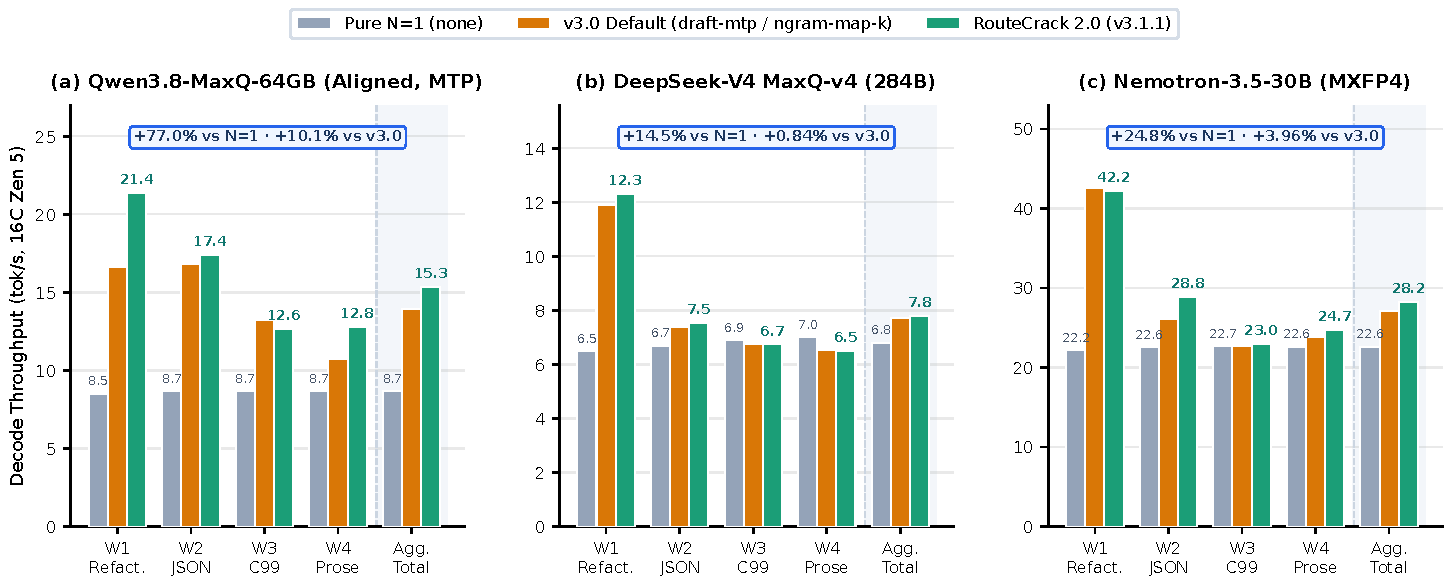
\includegraphics[width=\textwidth]{figures/fig3_routecrack2_speedup.pdf}
\caption{Per-workload and aggregate decode throughput of \texttt{RouteCrack 2.0} (\texttt{v3.1.1}) vs.\ Pure $N=1$ and \texttt{v3.0} speculators across \texttt{W1} (Refactor), \texttt{W2} (JSON Tools), \texttt{W3} (C99), \texttt{W4} (Prose), and Aggregate on 16 Zen~5 cores (0~GPU, $T=0$; \texttt{Nemotron} measured on \texttt{Fractal-MXFP4} reference).}
\label{fig:rc2}
\end{figure*}

\begin{table*}[t]
\centering
\caption{Cross-platform verification of \texttt{llama-modchip} across x86-64, Apple Silicon Metal, ARM64 cloud CPUs, and Vulkan hybrids (community runs cite their GitHub issue/PR).}
\label{tab:platforms}
\scriptsize
\setlength{\tabcolsep}{2.6pt}
\begin{tabularx}{\textwidth}{@{}lLLlccc@{}}
\toprule
\textbf{Hardware Platform} & \textbf{Cores / GPU} & \textbf{Memory} & \textbf{Model \& Format} & \textbf{Prefill} & \textbf{Base / Cold} & \textbf{Spec. / W1} \\
\midrule
AMD Ryzen 9 9955HX & 16C (Zen~5, AVX-512) & 60G cold cg (48.35, 0 reclaim) & \textbf{Qwen3.8 MaxQ-64GB} & \textbf{72--100} & 8.78 ($N=1$) & \textbf{15.64 / 22.00} \\
AMD Ryzen 9 9955HX & 16C (Zen~5, AVX-512) & 28.5G cold cg (28.26, 0 recl.) & \textbf{Qwen3.8 MaxQ-32GB} & \textbf{101--113} & 10.00 ($N=1$) & \textbf{14.58 / 15.31} \\
AMD Ryzen 9 9955HX & 16C (Zen~5, AVX-512) & 74G host (60G cg: ARC recl.) & \textbf{DS-V4 284B MaxQ-v4} & \textbf{45--50.5} & 6.80 ($N=1$) & \textbf{7.79 / 12.31} \\
AMD Ryzen 9 9955HX & 16C (Zen~5, AVX-512) & 15G cold cg ($N$=1; RC2 recl.) & \textbf{Nemotron MaxQ-16GB} & \textbf{188.3} & 22.64 ($N=1$) & \textbf{26.28$^\ddagger$ / 43.53} \\
Apple M5 Max & 18C CPU + 40C Metal GPU & 64 GB LPDDR5X (0 Swap) & DS-V4 \textit{legacy Fractal}$^*$ & 169.4 & 27.00 (\texttt{tg128}) & 20.7--23.6 \\
Threadripper 7985WX (\#1) & 64C (8 CCDs, 256 MB L3) & 256 GB 8-Ch DDR5 & Nemotron \texttt{Q4\_0} (\texttt{-t 32}) & \textbf{386.0} & 73.8--80.1 & \textbf{111.62 t/s} \\
Threadripper 9960X (\#40) & 24C (4 CCDs, AVX-512) & 125 GB 4-Ch DDR5 & Nemotron \texttt{VQ3-64} & \textbf{450.4} & 49.25 t/s & \textbf{54.43 t/s} \\
7945HX3D + RX 9070 XT & 16C + 16 GB Vulkan & 94 GB DDR5 + 16 GB & Nemotron (\texttt{MXFP4}) & \textbf{563.0} & 75.10 t/s & \textbf{80.80} (256K) \\
Apple M3/M4 Max (\#24,\#8) & ARM64 NEON + Metal & 36--64 GB Unified & Nemotron (\texttt{Frac}/\texttt{Q4}) & \textbf{860.1} & 71.6--78.6 & \textbf{236--250} (\texttt{RC2}) \\
AWS Graviton3 \texttt{m7g.2xl} (\#2) & 8 vCPU Neoverse-V1 & 31 GB DDR5 (0 GPU) & Nemotron-30B (\texttt{-t 8}) & \textbf{101.7} & 41.05 t/s & \textbf{44.97 t/s} \\
\bottomrule
\end{tabularx}
\vspace{2pt}
\raggedright\scriptsize $^*$Historical M5 Max result (\texttt{apple-silicon/results/dsv4-m5max.md}) was measured on the retired 56.56~GiB \texttt{DeepSeek-V4-Fractal} build, not \texttt{MaxQ-v4}; \texttt{MaxQ-v4} awaits fresh M5 Max re-measurement. $^\ddagger$\texttt{MaxQ-16GB} \texttt{RC2} at 15G cgroup refaulted ${\approx}9$~GiB/run from host ZFS ARC; bare-metal 16~GB \texttt{RC2} throughput at \texttt{-c 32768} is unverified. All prefill/decode rates in tok/s.
\end{table*}

\paragraph{Cold-Cache Cgroup v2 Evaluation Across All 4 Flagships (\texttt{Swap=0}, $n=3$ Cold Restarts).}
To test tier residency without warm outside-cgroup page cache and obtain valid i.i.d.\ variance (zero Stockfish TT carryover), we executed $n=3$ independent cold-server restarts per configuration (\texttt{-c 32768}, \texttt{-t 16 -tb 16}, \texttt{cache\_prompt=False}) after hypervisor \texttt{drop\_caches=3} + \texttt{POSIX\_FADV\_DONTNEED} (guest \texttt{Cached = 0.3~GiB} at start) inside strict transient \texttt{systemd-run} scopes (\texttt{MemoryAccounting=yes}, \texttt{MemorySwapMax=0}, 95\% Student-$t$ CIs with $\text{df}=2$, $t_{0.975,2}=4.303$). All 24 cold runs completed with \texttt{memory.swap.peak = 0~B} and \texttt{oom\_kill = 0}, separating into two clear regimes:
\emph{Strictly below cap (zero reclaim, certified):}
(i)~\textbf{\texttt{Qwen3.8 MaxQ-64GB}} (\texttt{MemoryMax=60G}, \texttt{qwen38\_64gb\_cgroup60g\_v311.json}): $N=1$ \textbf{8.78 $\pm$ 0.02~tok/s} (CI $\pm 0.05$, \texttt{VmHWM 45.46}, \texttt{cg.peak 46.53~GiB}) vs.\ \texttt{RC2} \textbf{15.64 $\pm$ 0.05~tok/s} (CI $\pm 0.11$, $+78.1\%$, \texttt{W1} 22.00 $\pm$ 0.19; \texttt{VmHWM 48.09}, \texttt{cg.peak 48.35~GiB}, \texttt{file 43.40~GiB}, \texttt{pgsteal=0}, \texttt{refault=0});
(ii)~\textbf{\texttt{Qwen3.8 MaxQ-32GB}} (\texttt{MemoryMax=28.5G}, \texttt{{-}{-}ctx-checkpoints 0}, hygiene sampling, \texttt{qwen38\_32gb\_cgroup28g\_v311.json}): $N=1$ \textbf{10.00 $\pm$ 0.01~tok/s} (\texttt{VmHWM 26.11}, \texttt{cg.peak 26.79~GiB}) vs.\ \texttt{RC2} \textbf{14.58 $\pm$ 0.32~tok/s} (CI $\pm 0.80$, $+45.8\%$, \texttt{W1} 15.31; \texttt{VmHWM 28.08}, \texttt{cg.peak 28.26~GiB}---tight 0.24~GiB headroom at 32K---with \texttt{file 25.14~GiB} out of 35.71~GiB on disk, proving \textbf{$>10.5$~GiB of PLE remained lazily unfaulted with \texttt{pgsteal=0}, \texttt{refault=0}});
(iii)~\textbf{\texttt{Nemotron MaxQ-16GB} $N=1$} (\texttt{MemoryMax=15G}, \texttt{nemotron\_16gb\_cgroup15g\_v311.json}): \textbf{22.64 $\pm$ 0.03~tok/s} (\texttt{VmHWM 14.92}, ${\approx}15.03$~GiB needed, 0.2~GiB refault---nearly fitting 15~GiB; higher than our earlier unpinned 15.10~t/s \texttt{llama-bench} \texttt{tg128} gate due to pinned 16C \texttt{taskset} + \texttt{q8\_0/q4\_0} KV).
\emph{Exceeds cap at \texttt{-c 32768} (OOM-free via ZFS-ARC-backed reclaim; bare-metal throughput unverified):}
(iv)~\textbf{\texttt{DeepSeek-V4 MaxQ-v4}} at \texttt{MemoryMax=60G} (\texttt{dsv4\_64gb\_cgroup60g\_v311.json}) requires ${\approx}60.3$--$60.7$~GiB ($57.99$~GiB weights $+ 2.25$--$2.67$~GiB anon), and \textbf{\texttt{MaxQ-16GB RC2}} at \texttt{MemoryMax=15G} requires ${\approx}15.75$~GiB ($13.39$~GiB $+ 2.36$~GiB anon). Both run without OOM/swap via continuous file-page reclaim (\texttt{DS-V4}: 10.7--30.7~GiB refaulted/run, 8.88 $\pm$ 0.25 \texttt{RC2} / 7.68 $\pm$ 0.01 $N=1$; \texttt{MaxQ-16GB RC2}: 8.4--9.2~GiB refaulted/run, 26.28 $\pm$ 0.19). Because refaults are served from our hypervisor host's ZFS ARC RAM rather than NVMe, those reclaim-bound rates do \emph{not} carry over to bare-metal 64/16~GB boxes without $\ge 61$~GiB (\texttt{DS-V4}) / $\ge 16$~GiB (\texttt{MaxQ-16GB RC2}) free RAM.

\paragraph{Single-Run Variance \& Honest Parity on Non-MTP Models.}
In Table~\ref{tab:rc2}, \texttt{Qwen3.8} gains $+77.0\%$ vs.\ $N=1$ and $+10.1\%$ vs.\ \texttt{v3.0 draft-mtp} ($+28.7\%$ on \texttt{W1} refactor via sub-250~ns suffix bypass and $+18.8\%$ on \texttt{W4} prose by curbing over-drafting). On non-MTP \texttt{DeepSeek-V4} ($+0.84\%$ vs.\ \texttt{v3.0}) and \texttt{Nemotron-30B} ($+3.96\%$ vs.\ \texttt{v3.0}), aggregate \texttt{RouteCrack 2.0} speed is effectively at parity with \texttt{v3.0 ngram-map-k} within single-run variance; its primary advantage on non-MTP models is eliminating \texttt{v3.0}'s \texttt{W2} JSON mode-bleed divergence and lifting \texttt{Nemotron W2} by $+10.5\%$ (28.83 vs.\ 26.08~tok/s).

\paragraph{Full Greedy $T=0$ Output Parity Disclosure (\texttt{identity\_vs\_n1}).}
Table~\ref{tab:identity} reports complete exact-prefix token match counts across all four workloads against $N=1$ greedy decoding. Across all three model families, \texttt{RouteCrack 2.0} achieves 100\% greedy bit-exact parity on structured \texttt{W1+W2} (fixing \texttt{v3.0}'s \texttt{W2} divergence on \texttt{DeepSeek} 120/191 and \texttt{Nemotron} 57/255 via 28-bit Tagged Mode Refutation). On high-entropy \texttt{W3}/\texttt{W4}, \emph{all} speculative methods---including \texttt{MTP-1} and \texttt{v3.0 draft-mtp}---diverge from $N=1$ at near-tied logits, which we attribute to batched verification GEMM (\texttt{batch > 1}) vs.\ $N=1$ GEMV FP32 FMA accumulation order (not yet isolated with a deterministic-reduction kernel).

\begin{table}[t]
\centering
\caption{Complete greedy $T=0$ common-prefix token parity vs.\ Pure $N=1$ (\texttt{identity\_vs\_n1} from raw \texttt{*\_routecrack2\_v31.json} logs).}
\label{tab:identity}
\scriptsize
\setlength{\tabcolsep}{3.2pt}
\begin{tabularx}{\columnwidth}{@{}lLcccc@{}}
\toprule
\textbf{Model} & \textbf{Speculator} & \textbf{W1} & \textbf{W2} & \textbf{W3} & \textbf{W4} \\
\midrule
\texttt{Qwen3.8} & \texttt{MTP-1} / \texttt{v3.0} & 254/254 & 254/254 & 4/254 & 79/254 \\
\texttt{Qwen3.8} & \textbf{\texttt{RouteCrack 2.0}} & \textbf{254/254} & \textbf{254/254} & 4/254 & 48/254 \\
\midrule
\texttt{DS-V4} & \texttt{v3.0} (\texttt{ngram-map}) & 191/191 & 120/191 & 53/191 & 48/191 \\
\texttt{DS-V4} & \textbf{\texttt{RouteCrack 2.0}} & \textbf{191/191} & \textbf{191/191} & 34/191 & 48/191 \\
\midrule
\texttt{Nemotron} & \texttt{v3.0} (\texttt{ngram-map}) & 255/255 & 57/255 & 17/253 & 134/255 \\
\texttt{Nemotron} & \textbf{\texttt{RouteCrack 2.0}} & \textbf{255/255} & \textbf{255/255} & 17/253 & 173/255 \\
\bottomrule
\end{tabularx}
\end{table}

\subsection{Cross-Platform Multi-ISA Verification}
Table~\ref{tab:platforms} summarizes local reference runs and community-submitted scorecards (GitHub Issues~\#1, \#2, \#8, \#16, \#40, PR~\#24) across x86-64, Apple Silicon Metal, ARM64 Neoverse-V1, and Vulkan hybrids.

\section{Limitations \& Engineering Trade-offs}
\begin{enumerate}
    \item \textbf{Loader \& Custom Kernel Portability}: Only \texttt{Nemotron MaxQ-16GB} ($\le 42$, 0 custom types, 0 ConeCollapse bias) targets unmodified upstream \texttt{llama.cpp} (\texttt{de32b268c+}) and downstream runners supporting \texttt{GGML\_TYPE\_Q2\_0 = 42}. \texttt{Qwen3.8 MaxQ-64GB} uses standard types $\le 42$ (pass \texttt{{-}{-}no-repack} on unpatched upstream \texttt{llama.cpp}). \texttt{Qwen3.8 MaxQ-32GB} and \texttt{DeepSeek-V4 MaxQ-v4} avoid custom tensor types for multi-backend portability but require \texttt{llama-modchip v3.1.1+} to load \texttt{ConeCollapse} \texttt{ffn\_down\_exps.bias}. Custom \texttt{FRACTAL\_64} (44) ships CPU and Apple Metal shaders and \texttt{VQ3\_64} (45) ships CPU SIMD kernels only (neither has CUDA/Vulkan shaders).
    \item \textbf{High-Entropy Prose on 284B Non-MTP MoE}: On \texttt{DeepSeek-V4 MaxQ-v4}, \texttt{W4} free prose runs $-7.4\%$ slower than $N=1$ (6.49 vs.\ 7.01~tok/s) because 256-expert DDR5 pull cost dominates whenever context n-grams miss; aggregate throughput still rises $+14.5\%$ via $+90.0\%$ \texttt{W1} and $+12.7\%$ \texttt{W2} gains.
    \item \textbf{Low-Bit Sampling Hygiene on \texttt{MaxQ-32GB}}: At 1.63~bpw, greedy $T=0$ sampling can trigger tail repetitions on long generations; applying \texttt{{-}{-}temp 0.6 {-}{-}top-p 0.95 {-}{-}top-k 20 {-}{-}presence-penalty 0.2 {-}{-}repeat-penalty 1.05} (automated by \texttt{./modchip}) restores loop-free generation.
\end{enumerate}

\section{Conclusion}
\texttt{llama-modchip v3.2.0} demonstrates that co-designing donor-free \texttt{MaxQ} compression (\texttt{PCA-Wiener + RaBitQ Q1\_0} PLE, FP64 Woodbury DualGram, and \texttt{ConeCollapse}), a zero-collision multi-ISA \texttt{ggml} ABI (\texttt{44}/\texttt{45}), zero-copy 3D MoE \texttt{{-}{-}repack}, Quantized Split-KV Decode, Native C++ Chained-Prefix HARP-Cache v2, and the \texttt{RouteCrack 2.0} 832~B L1 Micro-Arbiter enables 30B--284B Sparse MoE inference on commodity 16~GB, 32~GB, and 64~GB CPU workstations. Source code, unified patches, preflight verification tools, and raw benchmark artifacts are published under Apache~2.0 at \url{https://github.com/synchopate/llama-modchip}.

\FloatBarrier
\raggedbottom
{\small
\begin{thebibliography}{23}
\setlength{\itemsep}{1.5pt}
\setlength{\parskip}{0pt}

\bibitem{qwen38}
Qwen Team, ``Qwen3.8-Flash-Next Model Release,'' Hugging Face, \url{https://huggingface.co/Qwen/Qwen3.8-Flash-Next}, 2026.

\bibitem{deepseekv4}
DeepSeek-AI, ``DeepSeek-V4-Flash-0731 Model Release,'' Hugging Face, \url{https://huggingface.co/deepseek-ai/DeepSeek-V4-Flash-0731}, 2026.

\bibitem{deepseekv3}
DeepSeek-AI, ``DeepSeek-V3 Technical Report,'' \emph{arXiv preprint arXiv:2412.19437}, 2024.

\bibitem{nemotron35}
NVIDIA, ``NVIDIA-Nemotron-3.5-Lightning-30B-A3B Model Release,'' Hugging Face, \url{https://huggingface.co/nvidia/NVIDIA-Nemotron-3.5-Lightning-30B-A3B-BF16}, 2026.

\bibitem{nemotron2025}
NVIDIA, ``Nemotron-H: A Family of Accurate, Efficient Hybrid Mamba-Transformer Models,'' \emph{arXiv preprint arXiv:2504.03624}, 2025.

\bibitem{gloeckle2024mtp}
F.~Gloeckle, B.~Y.~Idrissi, B.~Rozi\`ere, D.~Lopez-Paz, and G.~Synnaeve, ``Better \& Faster Large Language Models via Multi-token Prediction,'' in \emph{Proc.\ ICML}, arXiv:2404.19737, 2024.

\bibitem{rabitq2024}
J.~Gao and C.~Long, ``RaBitQ: Quantizing High-Dimensional Vectors with a Theoretical Error Bound for Approximate Nearest Neighbor Search,'' in \emph{Proc.\ ACM SIGMOD}, arXiv:2405.12497, 2024.

\bibitem{llamacpp}
G.~Gerganov et al., ``\texttt{llama.cpp}: LLM Inference in C/C++,'' \url{https://github.com/ggml-org/llama.cpp}, 2023--2026.

\bibitem{frantar2023gptq}
E.~Frantar, S.~Ashkboos, T.~Hoefler, and D.~Alistarh, ``GPTQ: Accurate Post-Training Quantization for Generative Pre-trained Transformers,'' in \emph{Proc.\ ICLR}, arXiv:2210.17323, 2023.

\bibitem{lin2024awq}
J.~Lin, J.~Tang, H.~Tang, S.~Yang, W.-M.~Chen, W.-C.~Wang, G.~Xiao, X.~Dang, C.~Gan, and S.~Han, ``AWQ: Activation-aware Weight Quantization for LLM Compression and Acceleration,'' in \emph{Proc.\ MLSys}, arXiv:2306.00978, 2024.

\bibitem{tseng2024quip}
A.~Tseng, J.~Chee, Q.~Sun, V.~Kuleshov, and C.~De~Sa, ``QuIP\#: Even Better LLM Quantization with Hadamard Incoherence and Lattice Codebooks,'' in \emph{Proc.\ ICML}, arXiv:2402.04396, 2024.

\bibitem{egiazarian2024aqlm}
V.~Egiazarian, A.~Panferov, D.~Kuznedelev, E.~Frantar, A.~Babenko, and D.~Alistarh, ``Extreme Compression of Large Language Models via Additive Quantization,'' in \emph{Proc.\ ICML}, arXiv:2401.06118, 2024.

\bibitem{squeezellm}
S.~Kim, C.~Hooper, A.~Gholami, Z.~Dong, X.~Li, S.~Shen, M.~W.~Mahoney, and K.~Keutzer, ``SqueezeLLM: Dense-and-Sparse Quantization,'' in \emph{Proc.\ ICML}, arXiv:2306.07629, 2024.

\bibitem{dao2023flashattention2}
T.~Dao, ``FlashAttention-2: Faster Attention with Better Parallelism and Work Partitioning,'' in \emph{Proc.\ ICLR}, arXiv:2307.08691, 2024.

\bibitem{powerinfer}
Y.~Song, Z.~Mi, H.~Xie, and H.~Chen, ``PowerInfer: Fast Large Language Model Serving with a Consumer-Grade GPU,'' in \emph{Proc.\ ACM SOSP}, arXiv:2312.12456, 2024.

\bibitem{ktransformers}
H.~Chen et al., ``KTransformers: Unleashing the Full Potential of CPU/GPU Hybrid Inference for MoE Models,'' \url{https://github.com/kvcache-ai/ktransformers}, 2024--2026.

\bibitem{leviathan2023fast}
Y.~Leviathan, M.~Kalman, and Y.~Matias, ``Fast Inference from Transformers via Speculative Decoding,'' in \emph{Proc.\ ICML}, arXiv:2211.17192, 2023.

\bibitem{cai2024medusa}
T.~Cai, Y.~Li, Z.~Geng, H.~Peng, J.~D.~Lee, D.~Chen, and T.~Dao, ``Medusa: Simple LLM Inference Acceleration Framework with Multiple Decoding Heads,'' in \emph{Proc.\ ICML}, arXiv:2401.10774, 2024.

\bibitem{li2024eagle}
Y.~Li, F.~Wei, C.~Zhang, and H.~Zhang, ``EAGLE: Speculative Sampling Requires Rethinking Feature Uncertainty,'' in \emph{Proc.\ ICML}, arXiv:2401.15077, 2024.

\bibitem{fu2024lookahead}
Y.~Fu, P.~Bailis, I.~Stoica, and H.~Zhang, ``Break the Sequential Dependency of LLM Inference Using Lookahead Decoding,'' in \emph{Proc.\ ICML}, arXiv:2402.02057, 2024.

\bibitem{he2024rest}
Z.~He, Z.~Zhong, T.~Cai, J.~D.~Lee, and D.~He, ``REST: Retrieval-Based Speculative Decoding,'' in \emph{Proc.\ NAACL}, arXiv:2311.08252, 2024.

\bibitem{saxena2023promptlookup}
A.~Saxena, ``Prompt Lookup Decoding,'' \url{https://github.com/apoorvumang/prompt-lookup-decoding}, 2023.

\bibitem{stockfish}
T.~Romstad, M.~Costalba, J.~Kiiski, et al., ``Stockfish: Open-Source Chess Engine (Principal Variation Search and Zobrist Transposition Tables),'' \mbox{\url{https://stockfishchess.org}}, 2008--2026.

\end{thebibliography}
}

\end{document}
